As discussed in \autoref{sec:design-and-system-architecture}, the system is designed in FreeCAD \cite{freecad}, a parametric 3D modelling software. The below figures show the system in its entirety, with the front and back views of the system.

\begin{figure}[H]
    \hfill
    \begin{minipage}[h]{0.95\textwidth}
        \centering
        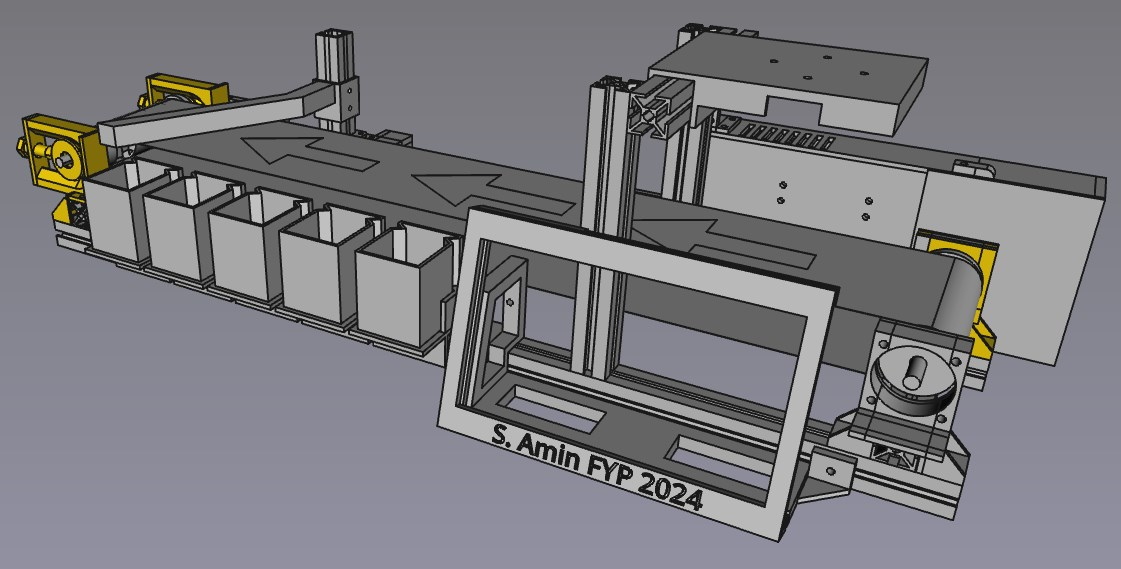
\includegraphics[width=\textwidth]{imgs/freecad/wholefront.jpg}
        \caption{Front View of the Mechanical Design}
    \end{minipage}
    \hfill
\end{figure}

The conveyor belt with the direction of travel is indicated with arrows. The camera is mounted on the top of the system, with LED lights inside the camera mount. The LCD mount for the DFRobot 7" LCD is clearly visible at the front, with a NEMA17 stepper motor mount positioned next to it for the driven conveyor rollers. The sorting bins are clearly present in the front of the system for easy user access.

\begin{figure}[H]
    \hfill
    \begin{minipage}[h]{0.95\textwidth}
        \centering
        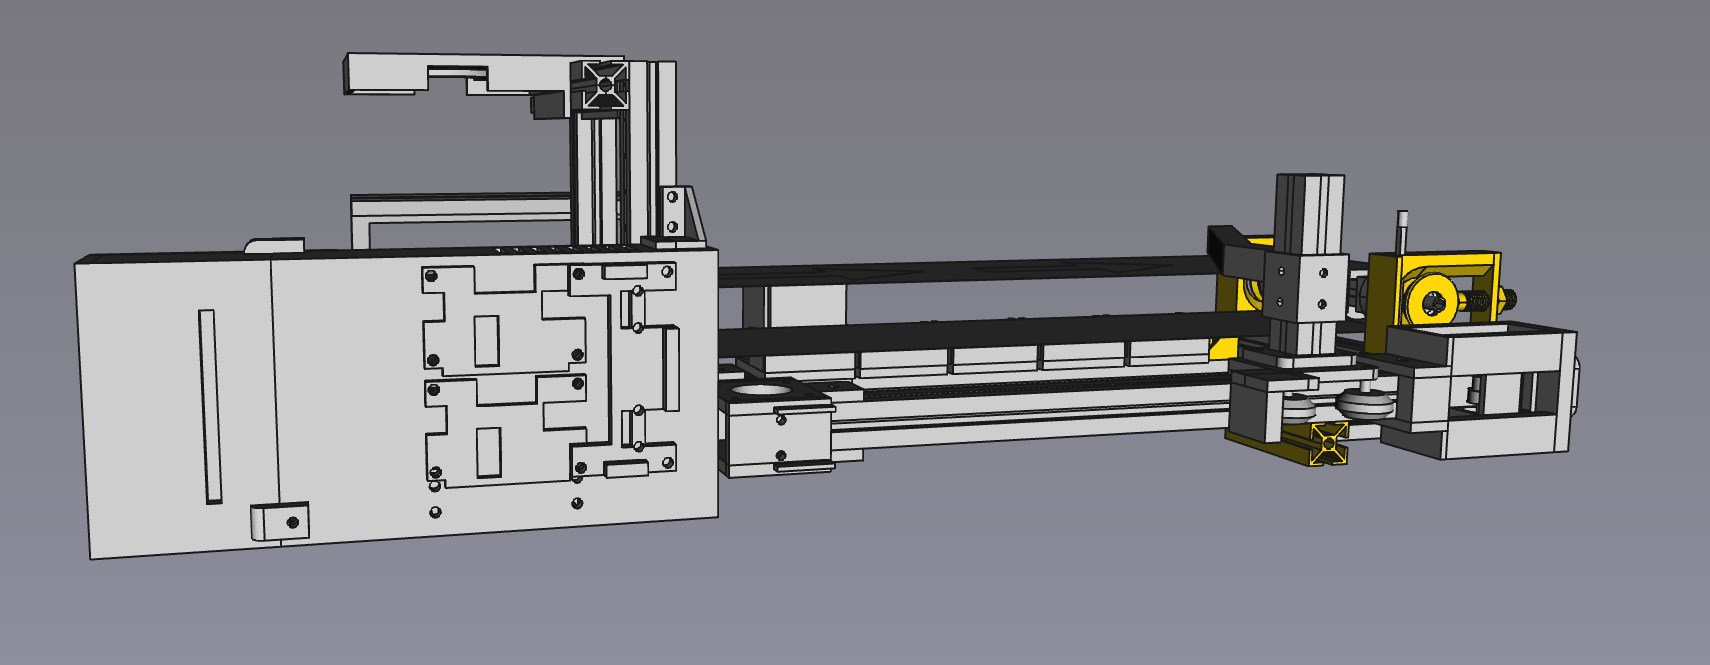
\includegraphics[width=\textwidth]{imgs/freecad/wholeback.jpg}
        \caption{Back View of the Mechanical Design}
    \end{minipage}
    \hfill
\end{figure}

From the back view of the system, the PSU enclosure is clearly visible with mounting plates for the step-down converters. A belt-driven arm is visible on the back, making use of another NEMA17 motor to drive it and a belt tensioner to ensure the belt is taut. The belt-driven arm is used to push components off the conveyor belt into the sorting bins. The tensioners for the conveyor belt itself are also visible in the back view on the right side.

\todo{show actual system}

\subsubsection{FDM Printer Settings}
\label{sec:3d-printer-settings}

As the system is using FDM printed parts, it is necessary to ensure that the parts are printed with the correct settings to give them the desired strength and durability. The parts are printed with a heavily modified Voxelab Aquila C2 FDM printer, with the following settings:


\begin{table}[H]
    \centering
    {\fontsize{10pt}{12pt}\selectfont
    \begin{tabularx}{\textwidth}{|p{3cm}|p{3cm}|X|}
        \hline
        \textbf{Setting} & \textbf{Value} & \textbf{Justification} \\
        \hline
        Layer Height & Dynamic (0.16-0.48 mm) & A dynamic layer height to balance quality and printing speed. The slicer will automatically adjust the layer height based on the required resolution of the current layer. \\
        \hline
        Wall Width & 1.8 mm & A 0.6 mm nozzle was used to increase printer speed, so the wall width is a multiple of the nozzle diameter. Three walls were chosen as a rule of thumb. \\
        \hline
        Infill Density & 16\% & The percentage of the part that is filled with extruded plastic. Higher infills are unnecessary as the parts are not load-bearing, and the air gaps for lower infills allow some flexibility in the parts. \\
        \hline
        Supports & 0\% Infill Tree Supports & Supports are required for 3D printed parts that have overhangs. Tree supports are used as they are easier to remove and use less material. The supports work well without infill due to the larger nozzle size. \\
        \hline
        Base Printing Speed & 72 mm/s & The speed at which the printer extrudes plastic. This was calculated from determining the printer's flow rate (maximum extrusion per second), the extrusion width and layer height. The speed was then set to 80\% of the maximum speed to ensure quality. The flow rate was determined to be 26mm$^3$/s, the layer height at its largest was 0.48mm, and the extrusion width was 0.6mm, from the above settings. Using the formula: \linebreak $Flow Rate = Layer Height \times Extrusion Width \times Speed$ \linebreak the maximum speed was determined to be 90mm/s, reduced to 80\% for quality, reaching 72mm/s. \\
        \hline
    \end{tabularx}
    }
    \caption{FDM Printer Settings}
    \label{tab:3dprintersettings}
\end{table}

\subsubsection{Power Supply Unit Enclosure}
\label{sec:power-supply-unit-enclosure}

Due to the potential of high-current carrying wires, the PSU has been enclosed in an FDM printed case, which prevents accidental contact with the PSU's terminals.

\begin{figure}[H]
    \hfill
    \begin{minipage}[h]{0.95\textwidth}
        \centering
        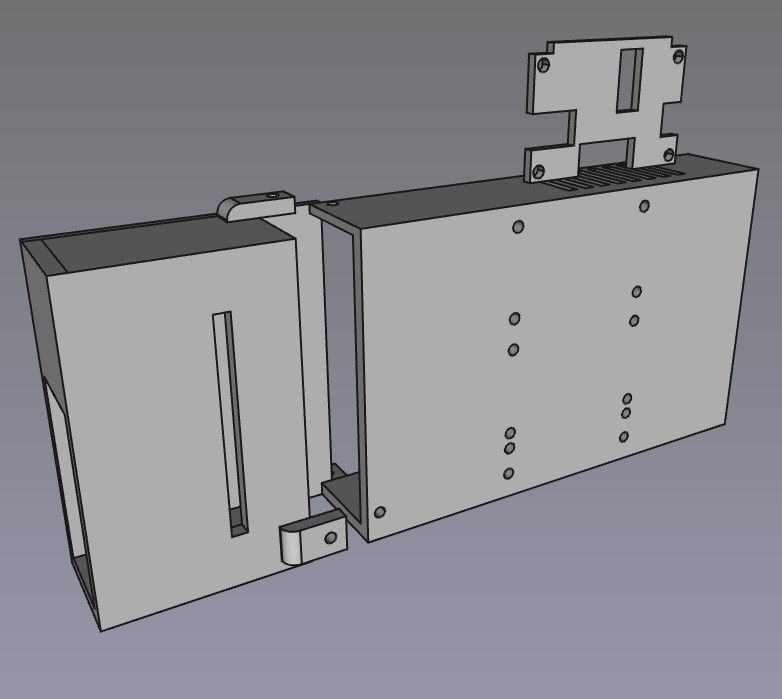
\includegraphics[height=8cm]{imgs/freecad/psu_mount.jpg}
        \caption{PSU Enclosure}
    \end{minipage}
    \hfill
\end{figure}

The PSU enclosure contains several components;
\textbf{PSU Container}: The PSU container is designed to house the 24V 6.25A power supply unit, and provides mounting holes for the other components. It attaches to the PSU using M3 screws.
\par
\textbf{Step-Down Converter Mounts}: The step-down converters are mounted on the PSU container using M3 screws. The step-down converters are used to convert the 24V output from the PSU to 12V and 5V for the system, shown by the two mounts at the top of the PSU container.
\par
\textbf{USB Breakout Mount}: For the 12V and 5V power outputs, a USB breakout board is used to provide power to the components, allowing standard cables to be used for power distribution. The USB breakout board is mounted on the right side of the PSU container, connecting to the step-down converters.
\par
\textbf{PSU Switch Housing}: For safety reasons, the connections between the switch and the PSU are enclosed in a housing to prevent accidental contact with the high voltage connections. There is a slot in the Switch Housing for the power cable to pass through to the step-down converters, and a switch snap-fit mount to hold the switch in place on the side.
\par
\textbf{PSU Mount}: The PSU mount is used to mount the PSU container to the 2020 extrusion frame of the system. The mount is screwed into the top of the PSU container and the 2020 extrusion frame, using M3 screws and T-nuts.

\begin{figure}[H]
    \hfill
    \begin{minipage}[h]{0.45\textwidth}
        \centering
        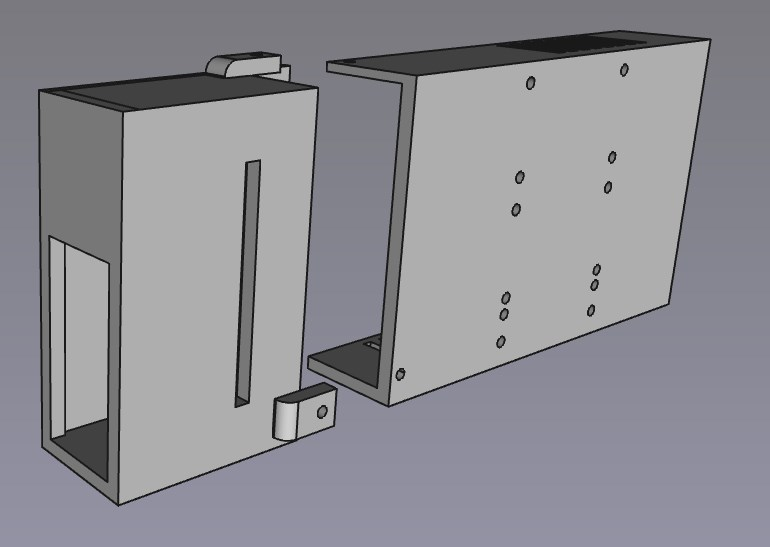
\includegraphics[height=6cm]{imgs/freecad/psu_switch.jpg}
        \caption{PSU Switch Housing}
    \end{minipage}
    \hfill
    \begin{minipage}[h]{0.45\textwidth}
        \centering
        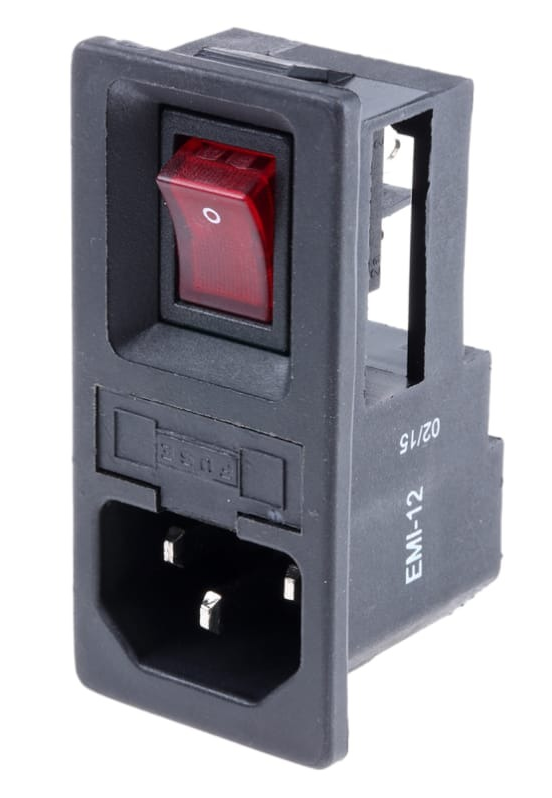
\includegraphics[height=6cm]{imgs/parts/iec_c14.jpg}
        \caption{IEC C14 Power Socket \cite{rsproc14switch}}
        \end{minipage}
    \hfill
\end{figure}

A standard IEC C14 power connector and an RS Pro Snap-In Fused Rocker Switch \cite{rsproc14switch} are used to connect the PSU to the mains power. As the power supply is a 6.25A power supply, a 6A fuse was chosen for the switch, which is the closest available fuse rating to the power supply's current rating. This ensures that the fuse will trigger before the power supply is damaged, should there be a short circuit in the system. For wiring the power supply and connecting the step-down converters, 18AWG wire was chosen which is rated for 17A \cite{18awgwire}, which is sufficient for the system's power consumption. The wire is securely crimped to the power supply using a crimping tool.

\begin{minipage}{\textwidth}
    \begin{minipage}{0.6\textwidth}
        \centering
        {\fontsize{10pt}{12pt}\selectfont
        \begin{tabularx}{\textwidth}{|X|p{1cm}|p{1cm}|X|}
            \hline
            \textbf{Test} & \textbf{Result} & \textbf{Req} & \textbf{Description} \\ \hline
            Earth Continuity & 0.06$\Omega$ & $\leq$ 0.1$\Omega$ & Verifies the earth wire is connected. \\ \hline
            Earth Leakage & 0.2mA & $\leq$ 0.75mA & Ensure the touchable metal parts cannot cause harm. \\ \hline
            Insulation Resistance & 320M$\Omega$ & $\geq$ 1M$\Omega$ & Ensure wires are sufficiently insulated. \\ \hline
        \end{tabularx}
        }
    \end{minipage}%
    \hfill % Adds horizontal space between the table and the image
    \begin{minipage}{0.45\textwidth}
        \centering
        \raisebox{-\height}{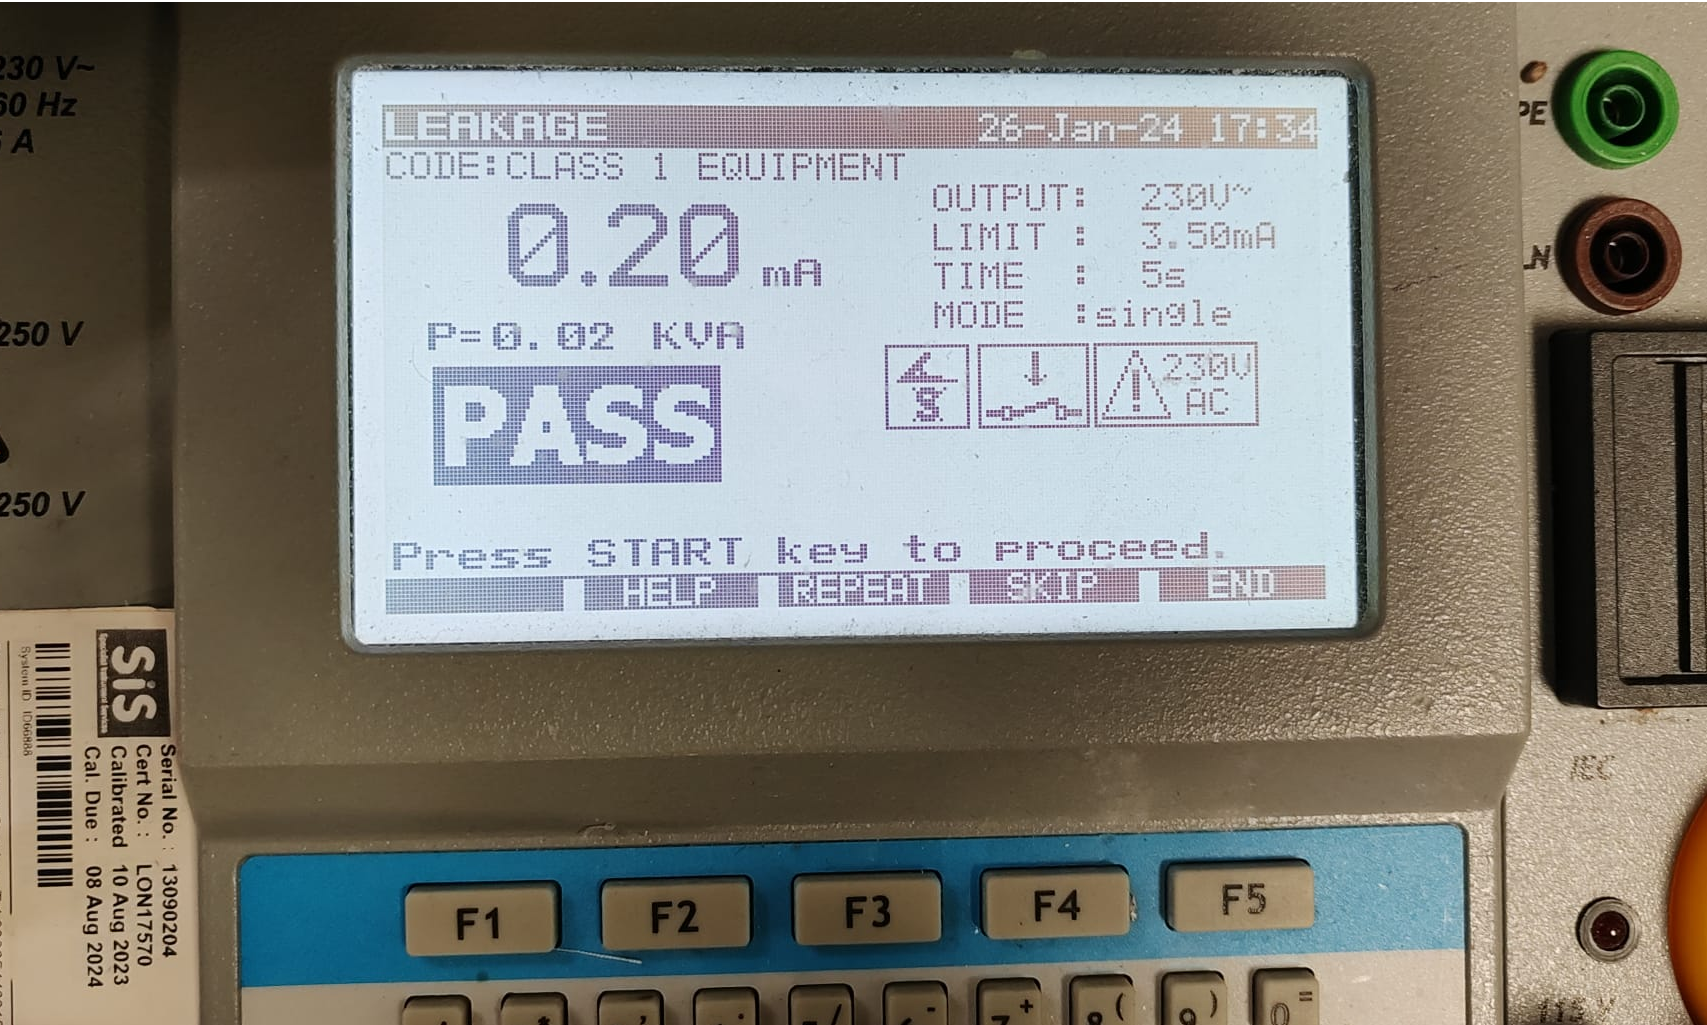
\includegraphics[height=3.5cm]{imgs/pattesting.jpeg}}
    \end{minipage}
    \captionof{table}{PAT Testing Results and PAT Machine}
    \label{tab:pat}
\end{minipage}


Due to the concern of electrical safety,  the power supply has been PAT tested by technicians in the Level 1 Labs and has been deemed safe for use. PAT (Portable Appliance Testing) is a process by which electrical appliances are routinely checked for safety \cite{patwiki, patspec}. The results of the PAT test are shown in \autoref{tab:pat}.

\begin{figure}[H]
    \begin{minipage}[h]{0.95\textwidth}
        \centering
        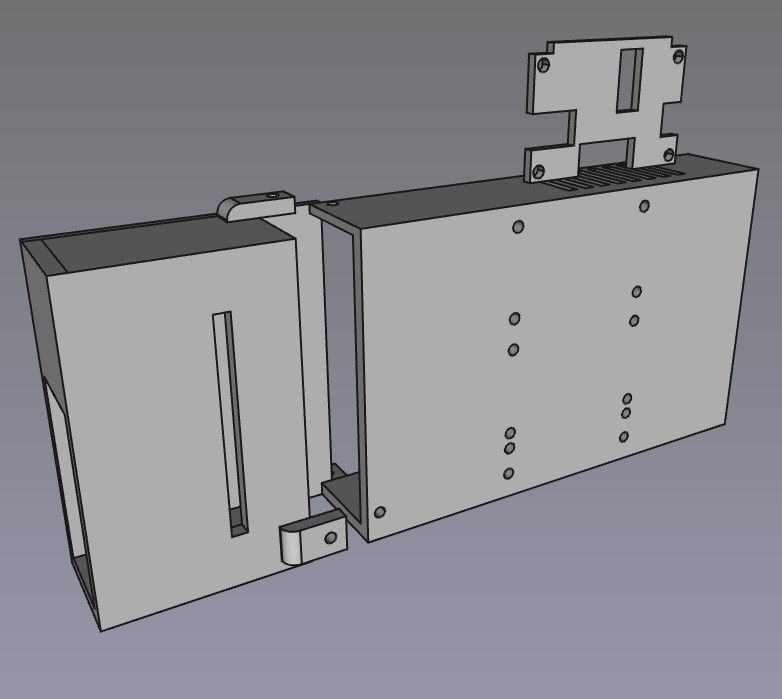
\includegraphics[height=8cm]{imgs/freecad/psu_mount.jpg}
        \caption{Final PSU Enclosure}
        \label{fig:psuenclosure}
    \end{minipage}
\end{figure}
\todo{show actual PSU}

As shown in \autoref{fig:psuenclosure}, the final PSU enclosure is shown to be working with the 5V and 12V outputs connected to the mounted USB breakout boards.

\subsubsection{LCD and Camera Mounts}
\label{sec:lcd-mount}
For the DFRobot 7" LCD, a mount was designed to hold the LCD in place on the front of the system. The LCD is affixed at a 15$^{\circ}$ angle to the front of the system, allowing for easy viewing by the user. The mount is designed to be attached to the 2020 extrusion frame of the system, using M3 screws and T-nuts.


\begin{figure}[H]
    \begin{minipage}[h]{0.95\textwidth}
        \centering
        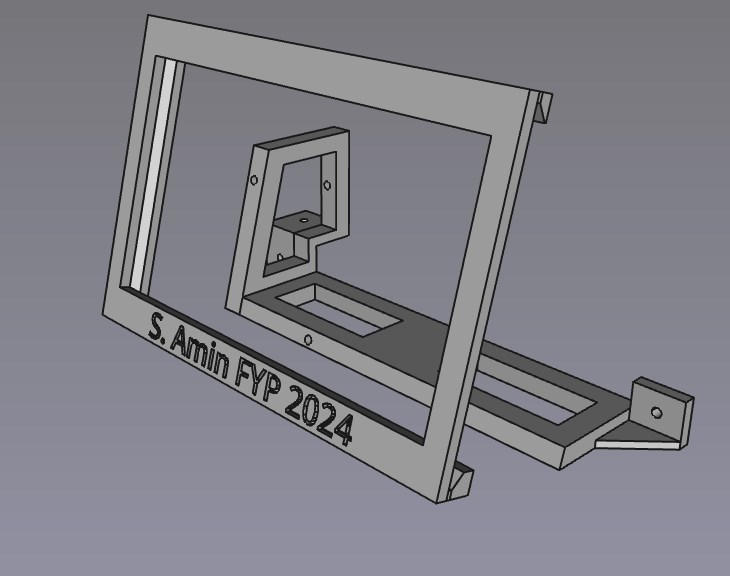
\includegraphics[height=8cm]{imgs/freecad/lcd_mount2.jpg}
        \caption{LCD Mount}
        \label{fig:lcdmount}
    \end{minipage}
\end{figure}

The design consists of two parts;
\textbf{LCD Cover}: The LCD cover is designed to hold the LCD in place. It contains a small gap that the LCD fits into, preventing it from falling out with the help of friction.
\par
\textbf{LCD Extrusion Mount}: The LCD extrusion mount is designed to be attached to the 2020 extrusion frame of the system. It contains screw holes for the LCD Cover to be attached to, and screw holes for the 2020 extrusion frame. It also contains a support for the LCD cover to rest on, preventing it from breaking off.


\begin{figure}[H]
    \begin{minipage}[h]{0.95\textwidth}
        \centering
        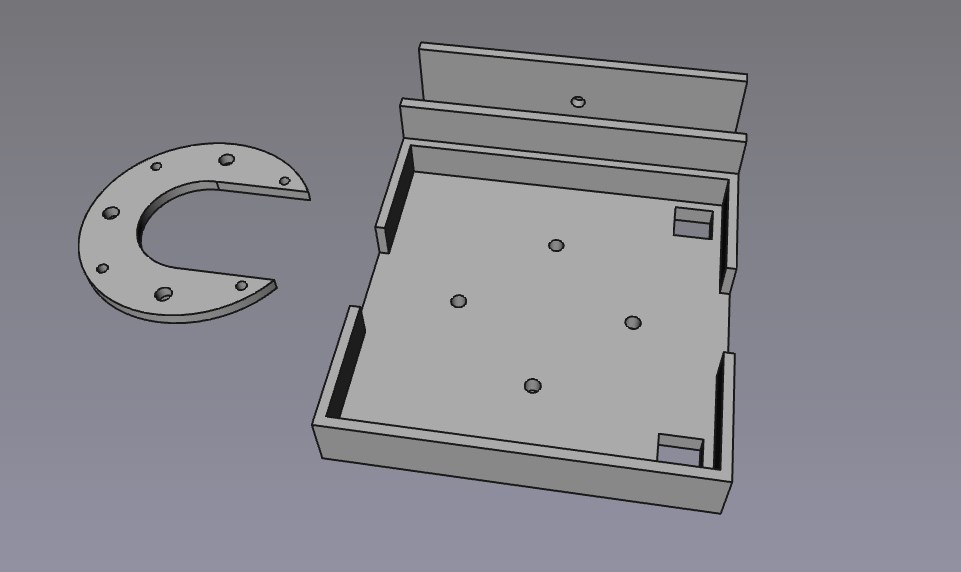
\includegraphics[height=8cm]{imgs/freecad/cameraplate.jpg}
        \caption{Camera mount and plate}
        \label{fig:cameraplate}
    \end{minipage}
\end{figure}

For the Okdo OV5647 Camera, a mount was designed to hold the camera face down above the conveyor belt. The camera is mounted on the top of the system, with LED lights inside the camera mount. The mount consists of two parts as shown in \autoref{fig:cameraplate};
\textbf{Extrusion Mount}: The extrusion mount is designed to be attached to the 2020 extrusion frame of the system. It contains a hole for the WS2812B LED strip wires to pass through, and screw holes for the camera plate to be attached to. The mount fits onto the extrusion, however this is not strictly necessary as the camera mount is able to fit on the extrusion without falling off.
\par
textbf{Camera Plate}: The camera plate is designed to hold the camera in place. It contains four holes for the Okdo OV5647 Camera to be attached to, and a slot for the camera ribbon cable to pass through, ensuring that the camera remains flat.
\subsubsection{Conveyor Belt}
\label{sec:conveyor-belt}
The conveyor belt is a key component of the system, as it is used to transport components from the input side to the bins. As such, it is the largest component of the system, and so makes use of 2020 aluminium extrusion as its skeleton. The conveyor belt has two rollers; one actively driven by a NEMA17 stepper motor, and the other is a free roller. The conveyor belt relies on friction to turn the idle roller, so it is essential that the belt is taut. To ensure this, belt tensioners are used on the idler side of the conveyor belt.

\begin{figure}[H]
    \begin{minipage}[h]{0.95\textwidth}
        \centering
        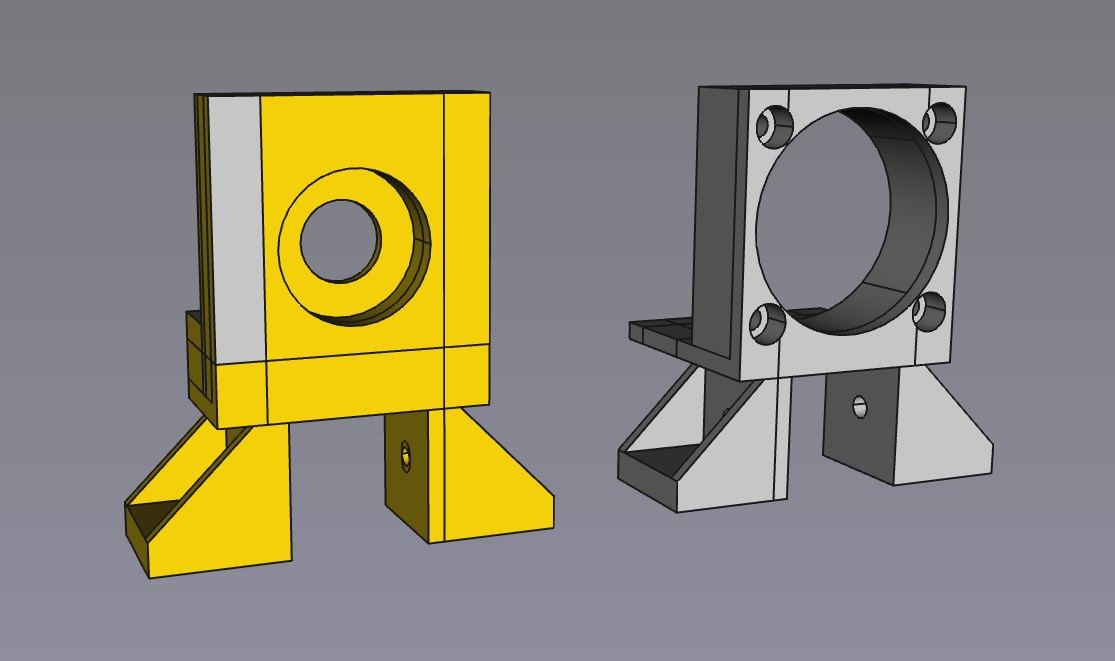
\includegraphics[height=8cm]{imgs/freecad/conveyor_driven.jpg}
        \caption{Driven Conveyor Roller}
        \label{fig:conveyordriven}
    \end{minipage}
\end{figure}

\autoref{fig:conveyordriven} shows the mounts for the driven conveyor roller, the right mount will mount the NEMA17 stepper through four M3 screws, and the left mount holds the other side of the roller by allowing it to rotate freely in the mount. The left mount contains a space for a 608ZZ bearing to be inserted, which allows the roller to rotate freely without friction (8x22x7mm). There is a clear 20x20mm slot for the 2020 extrusion frame to be inserted into, allowing the mounts to attach to the frame, securing it in place. The left mount can also be disassembled to allow for the belt and roller to  be inserted into the system easily.

\begin{figure}[H]
    \begin{minipage}[h]{0.95\textwidth}
        \centering
        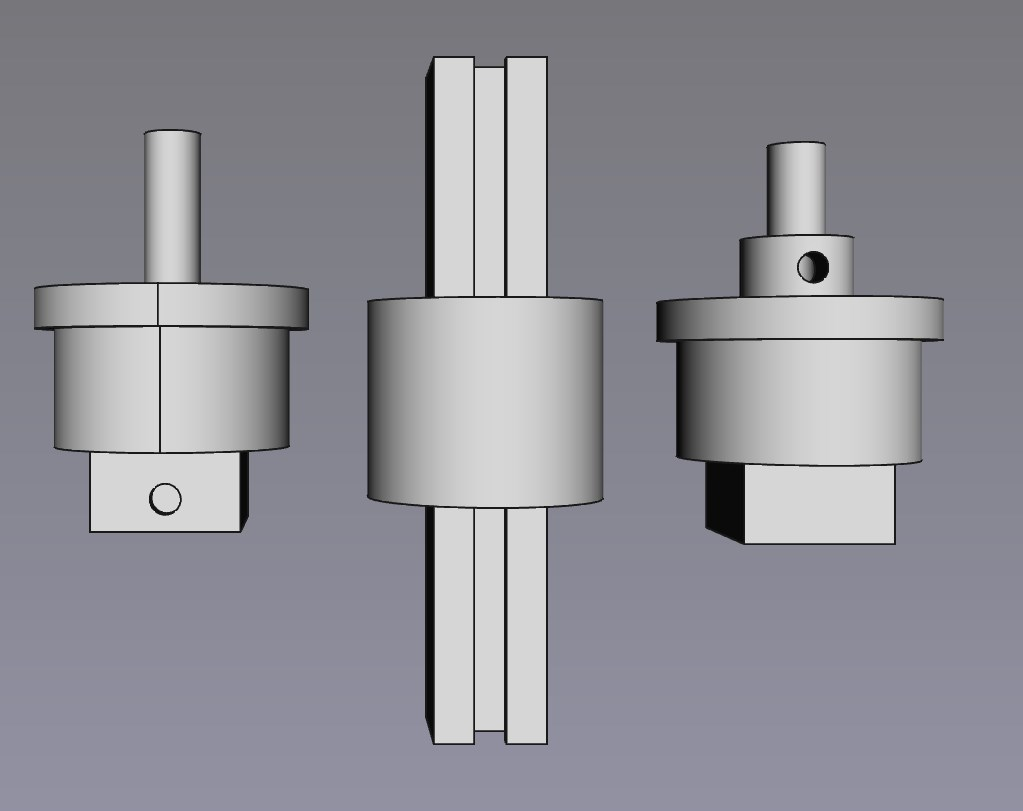
\includegraphics[height=8cm]{imgs/freecad/rollers.jpg}
        \caption{Conveyor Belt Rollers}
        \label{fig:conveyorrollers}
    \end{minipage}
\end{figure}

\autoref{fig:conveyorrollers} shows the rollers themselves, with non-driven end rollers on the left, the adjustable-length roller body in the middle, and the motor-coupled roller on the right. During initial development, it was unsure what the width of the conveyor belt would be, so a design was made to allow for the length of the rollers to be adjusted. This is done by using a screw on the roller ends to adjust where it locks onto the roller body, enabling the length of the roller to be adjusted. The roller is coupled to the motor by screwing an M3 screw into the side of the roller which pushes against the motor shaft, allowing the motor to drive the roller. \autoref{fig:adjustablerollers} shows the adjustable roller design.

\begin{figure}[H]
    \begin{minipage}[h]{\textwidth}
        \centering
        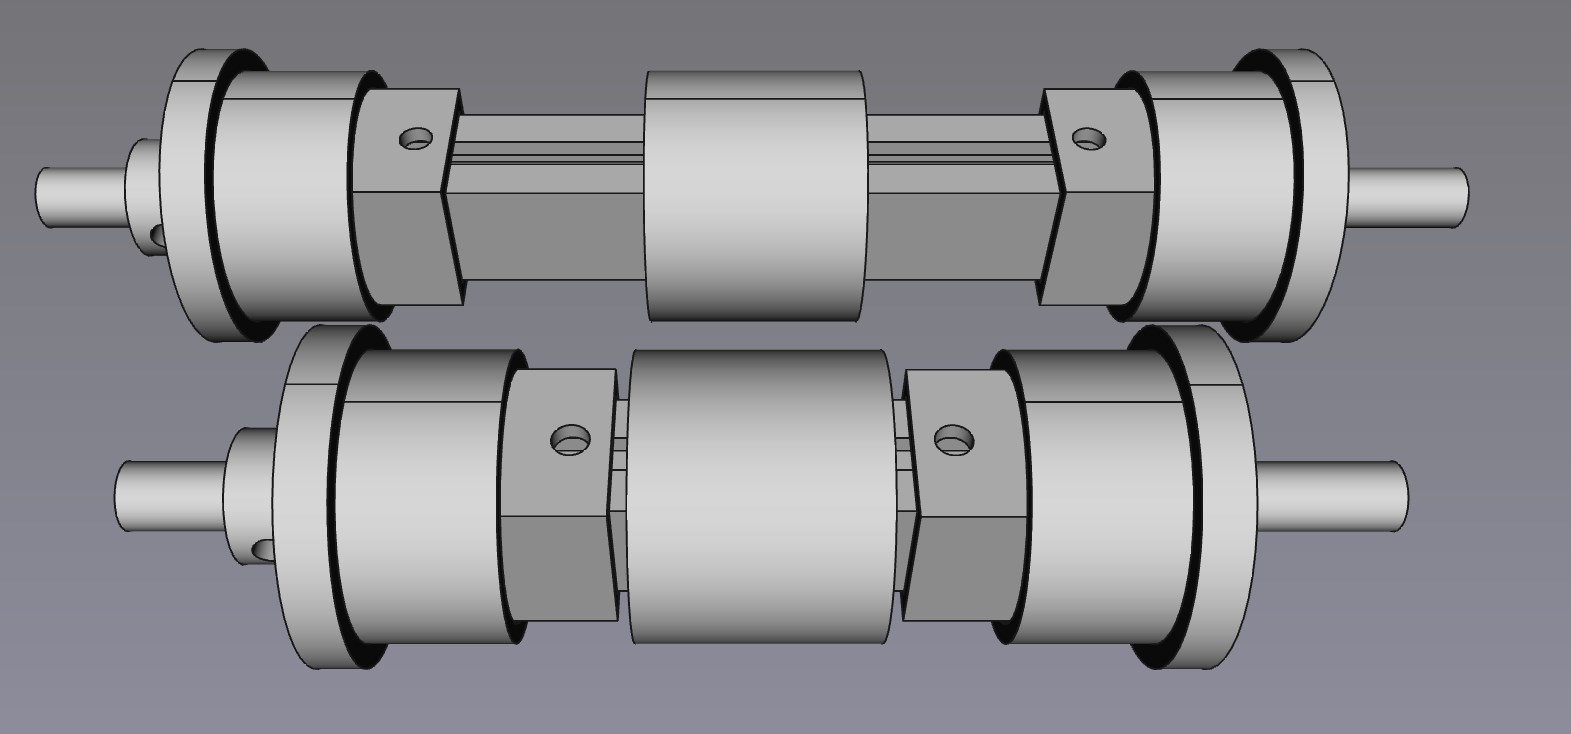
\includegraphics[height=8cm]{imgs/freecad/adjustablerollers.jpg}
        \caption{Adjustable Conveyor Rollers}
        \label{fig:adjustablerollers}
    \end{minipage}
\end{figure}

On the other side of the conveyor belt, the belt tensioner is used to ensure the belt is taut as shown in \autoref{fig:belttensioner}.

\begin{figure}[H]
    \begin{minipage}[h]{0.95\textwidth}
        \centering
        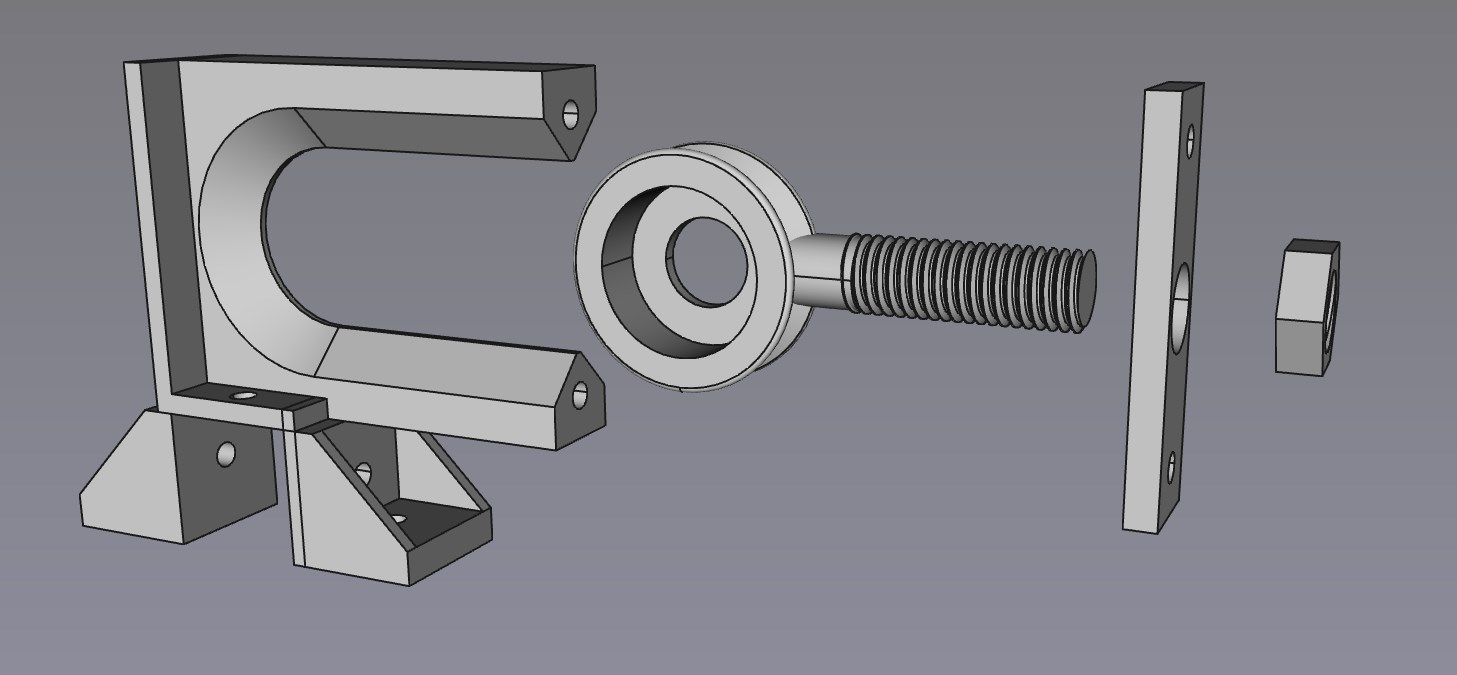
\includegraphics[width=\textwidth]{imgs/freecad/belttensioner.jpg}
        \caption{Belt tensioner design}
        \label{fig:belttensioner}
    \end{minipage}
\end{figure}

As usual, the belt tensioner is mounted to the 2020 extrusion frame using M3 screws and T-nuts. The tensioner is made of 4 distinct parts;
\textbf{Belt Tensioner Mount}: The mount is used to attach the tensioner to the 2020 extrusion frame. The mount contains a bevelled edge to allow the tensioner to slide in and out of the mount.
\par
\textbf{Belt Tensioner}: The tensioner is used to tension the conveyor belt. It slots into the mount, and features a 608ZZ bearing to allow the rollers to rotate freely. It is threaded to allow the belt tensioner nut to be screwed in.
\par
\textbf{Belt Tensioner Cover}: The cover is used to ensure that the tensioner does not slip out, and provides something for the nut to press against to tension the belt.
\par
\textbf{Belt Tensioner Nut}: The nut is used to tension the belt. It is screwed into the tensioner cover, and presses against the tensioner to tension the belt.

\begin{figure}[H]
    \begin{minipage}[h]{0.95\textwidth}
        \centering
        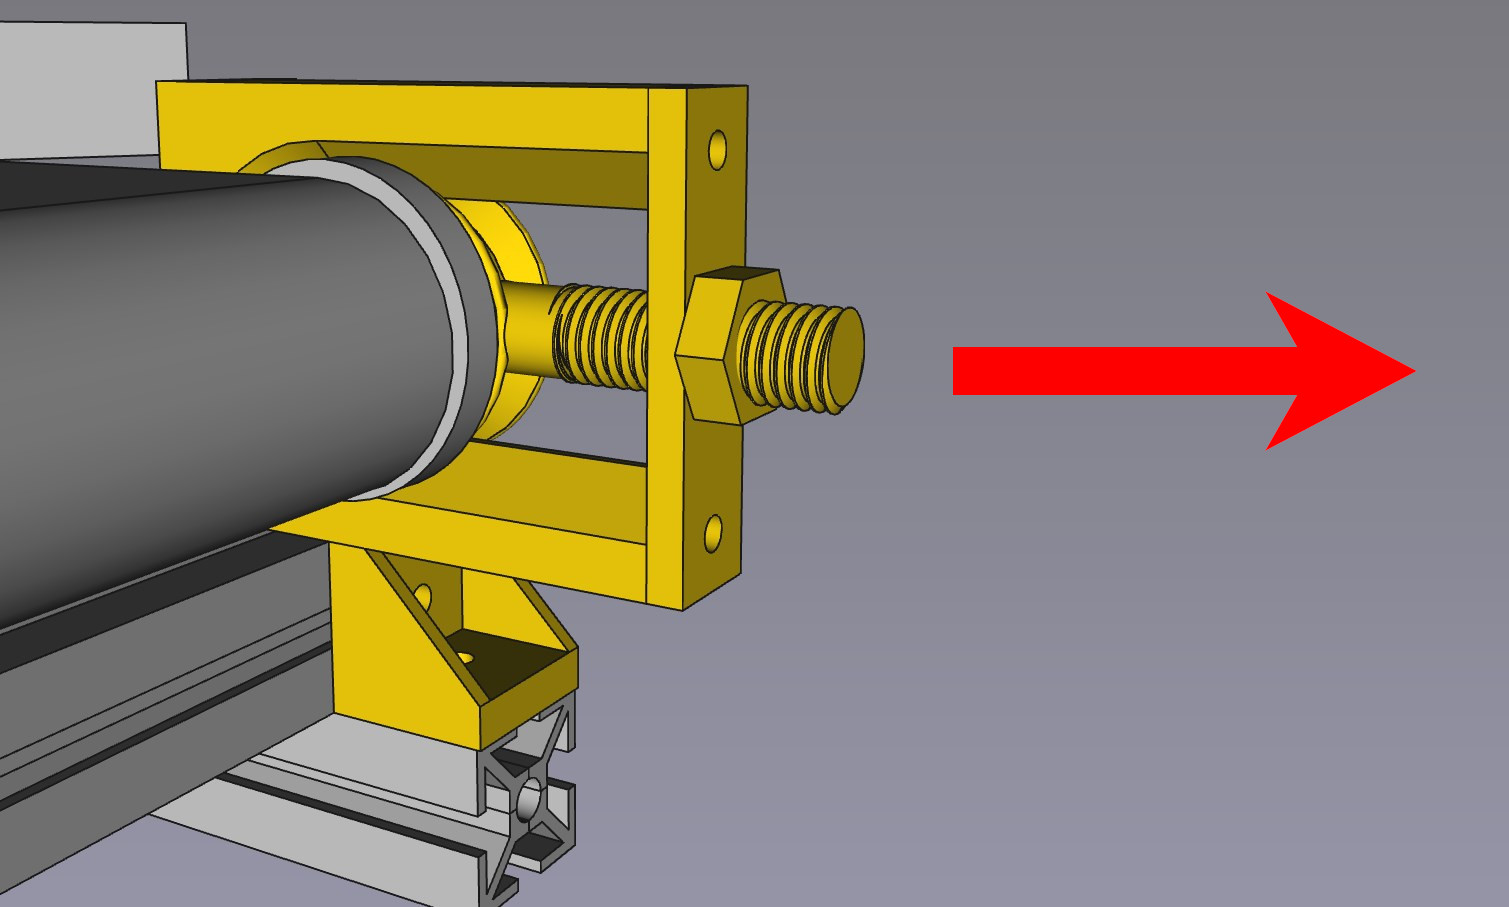
\includegraphics[height=8cm]{imgs/freecad/tensionerapplication.jpg}
        \caption{Belt tensioner in use}
        \label{fig:belttensioneractive}
    \end{minipage}
\end{figure}

To tension the belt, the nut is simply turned which forces the tensioner to retract or extend in the mount, tensioning the belt. As shown in \autoref{fig:belttensioneractive}, tightening the nut would force the tensioner to move in the direction of the arrow, causing the belt to be tensioned.

\subsubsection{Sweeping Mechanism}
The sweeping mechanism of the system contains many intricate parts. It is responsible for pushing components off the conveyor belt into the sorting bins. The mechanism is driven by a NEMA17 stepper motor, which is mounted to the 2020 extrusion frame of the system. The motor then drives a GT2 belt, which is connected to the sweeping arm, allowing it to move linearly down the length of the conveyor belt. 
\begin{figure}[H]
    \begin{minipage}[h]{0.95\textwidth}
        \centering
        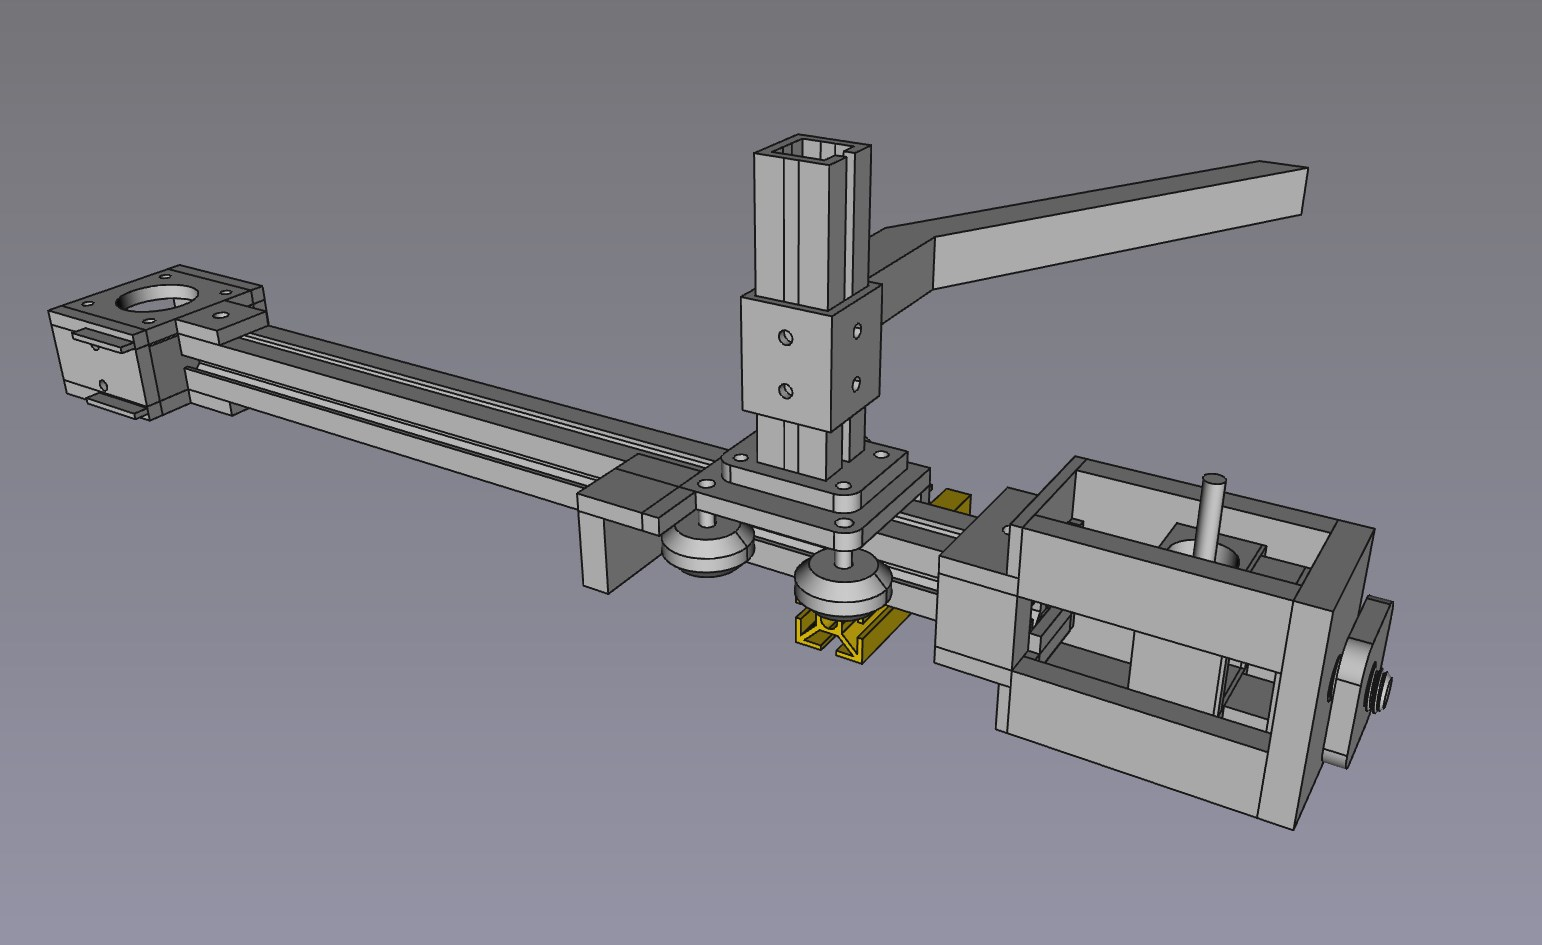
\includegraphics[height=8cm]{imgs/freecad/fullsweeper.jpg}
        \caption{Full Sweeping Mechanism}
        \label{fig:sweeperfull}
    \end{minipage}
\end{figure}

The arm makes use of v-rollers to move smoothly along the 2020 extrusion frame, inspired by traditional x-gantry designs of 3D printers, as shown in \autoref{fig:ender3}. The arm is mounted to the v-rollers using M3 screws and T-nuts, allowing it to be adjusted to the correct height.

\begin{figure}[H]
    \begin{minipage}[h]{0.95\textwidth}
        \centering
        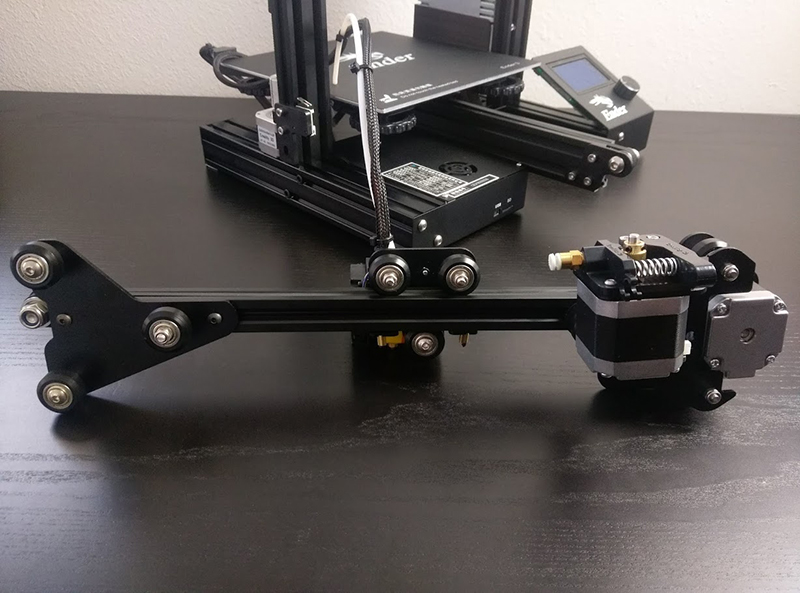
\includegraphics[height=8cm]{imgs/freecad/ender_3_assembly_x_axis_complete.jpg}
        \caption{Ender 3 X-Gantry \cite{brett_2018}}
        \label{fig:ender3}
    \end{minipage}
\end{figure}

The sweeper contains several parts;

\textbf{Motor and Endstop Mount}: The mount is used to attach the NEMA17 stepper motor to the 2020 extrusion frame. It contains four screw holes for the motor, and two screw holes for the endstop. The endstop is used to detect when the sweeper arm has reached the end of its travel, and is used to prevent the motor from damaging the system. This allows precise control of the sweeper arm's position. In \autoref{fig:motorandtensioner}, the motor and endstop mount is shown on the far left.
\par
\textbf{Belt Tensioner}: The belt tensioner is used to tension the GT2 belt that drives the sweeper arm. It is mounted to the 2020 extrusion frame using M3 screws and T-nuts, and contains a 608ZZ bearing to allow the belt to rotate freely. The tensioner is used to tension the belt, ensuring that the belt is taut and does not slip. This design is similar to the conveyor belt tensioner in that it uses a nut to tension the belt. Inside the tensioner, there is a GT2 gear that the belt wraps around, and it is affixed to a 5mm shaft that is allowed to rotate freely using two 608ZZ bearings. The tensioner is allowed to move in only direction as it is housed in a "container" --- similar to the conveyor belt tensioner. This is clearly shown in \autoref{fig:motorandtensioner}.

\begin{figure}[H]
    \hfill
    \begin{minipage}[t]{0.45\textwidth}
      \centering
      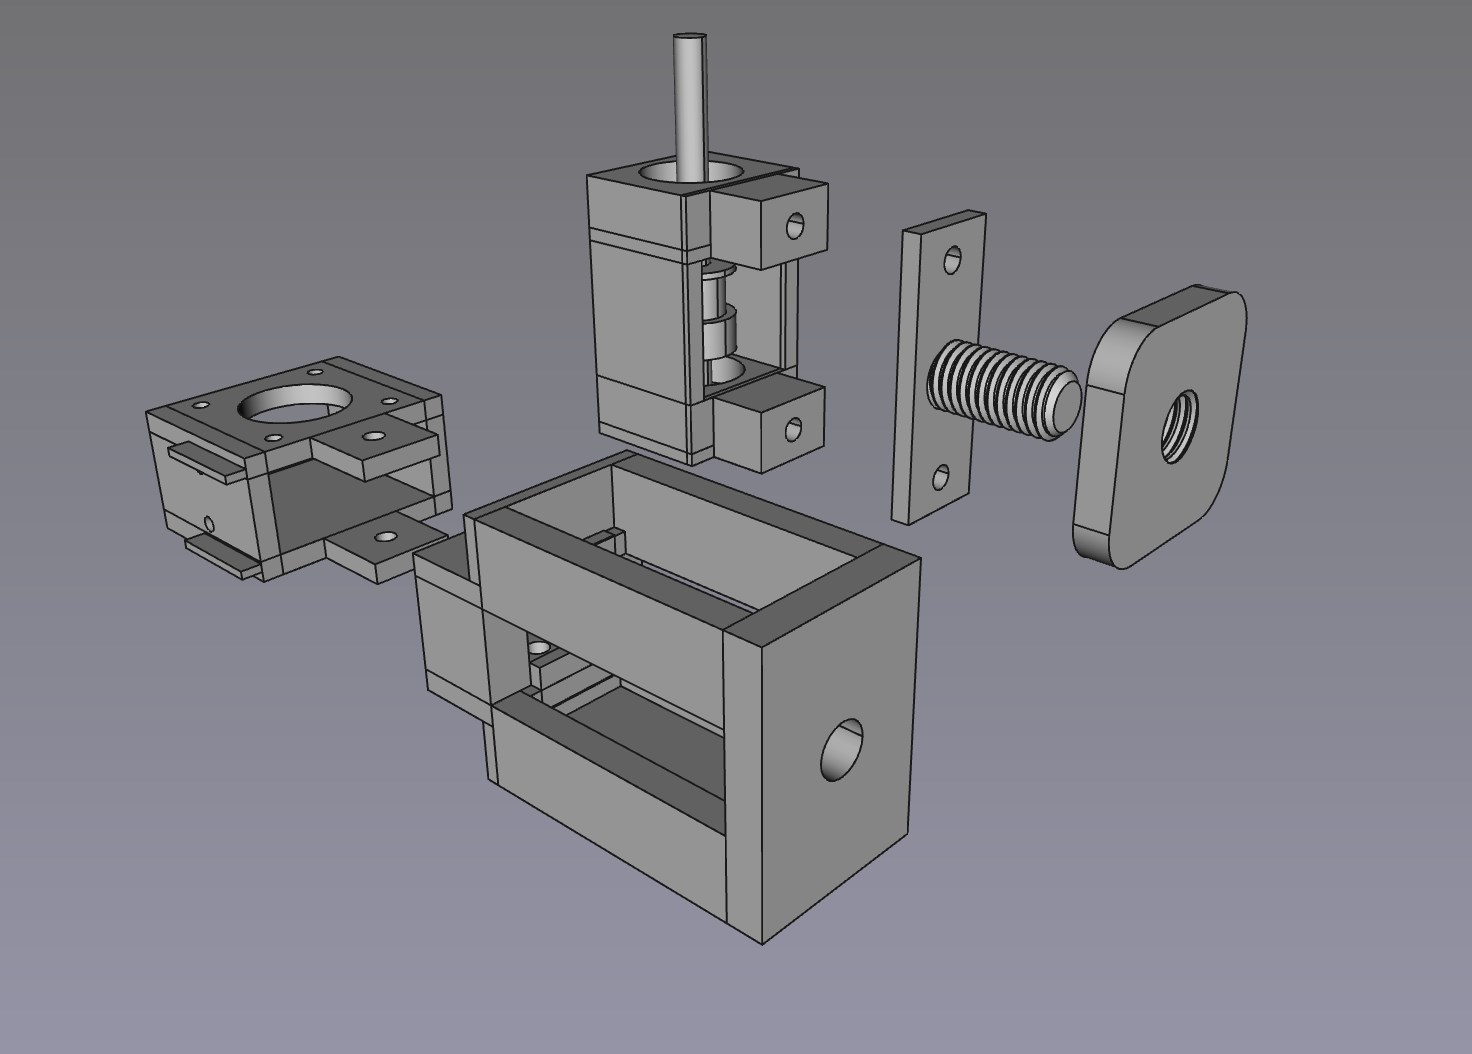
\includegraphics[height=7cm]{imgs/freecad/motorandtensioner.jpg}
    \end{minipage}
    \hfill
    \begin{minipage}[t]{0.45\textwidth}
      \centering
      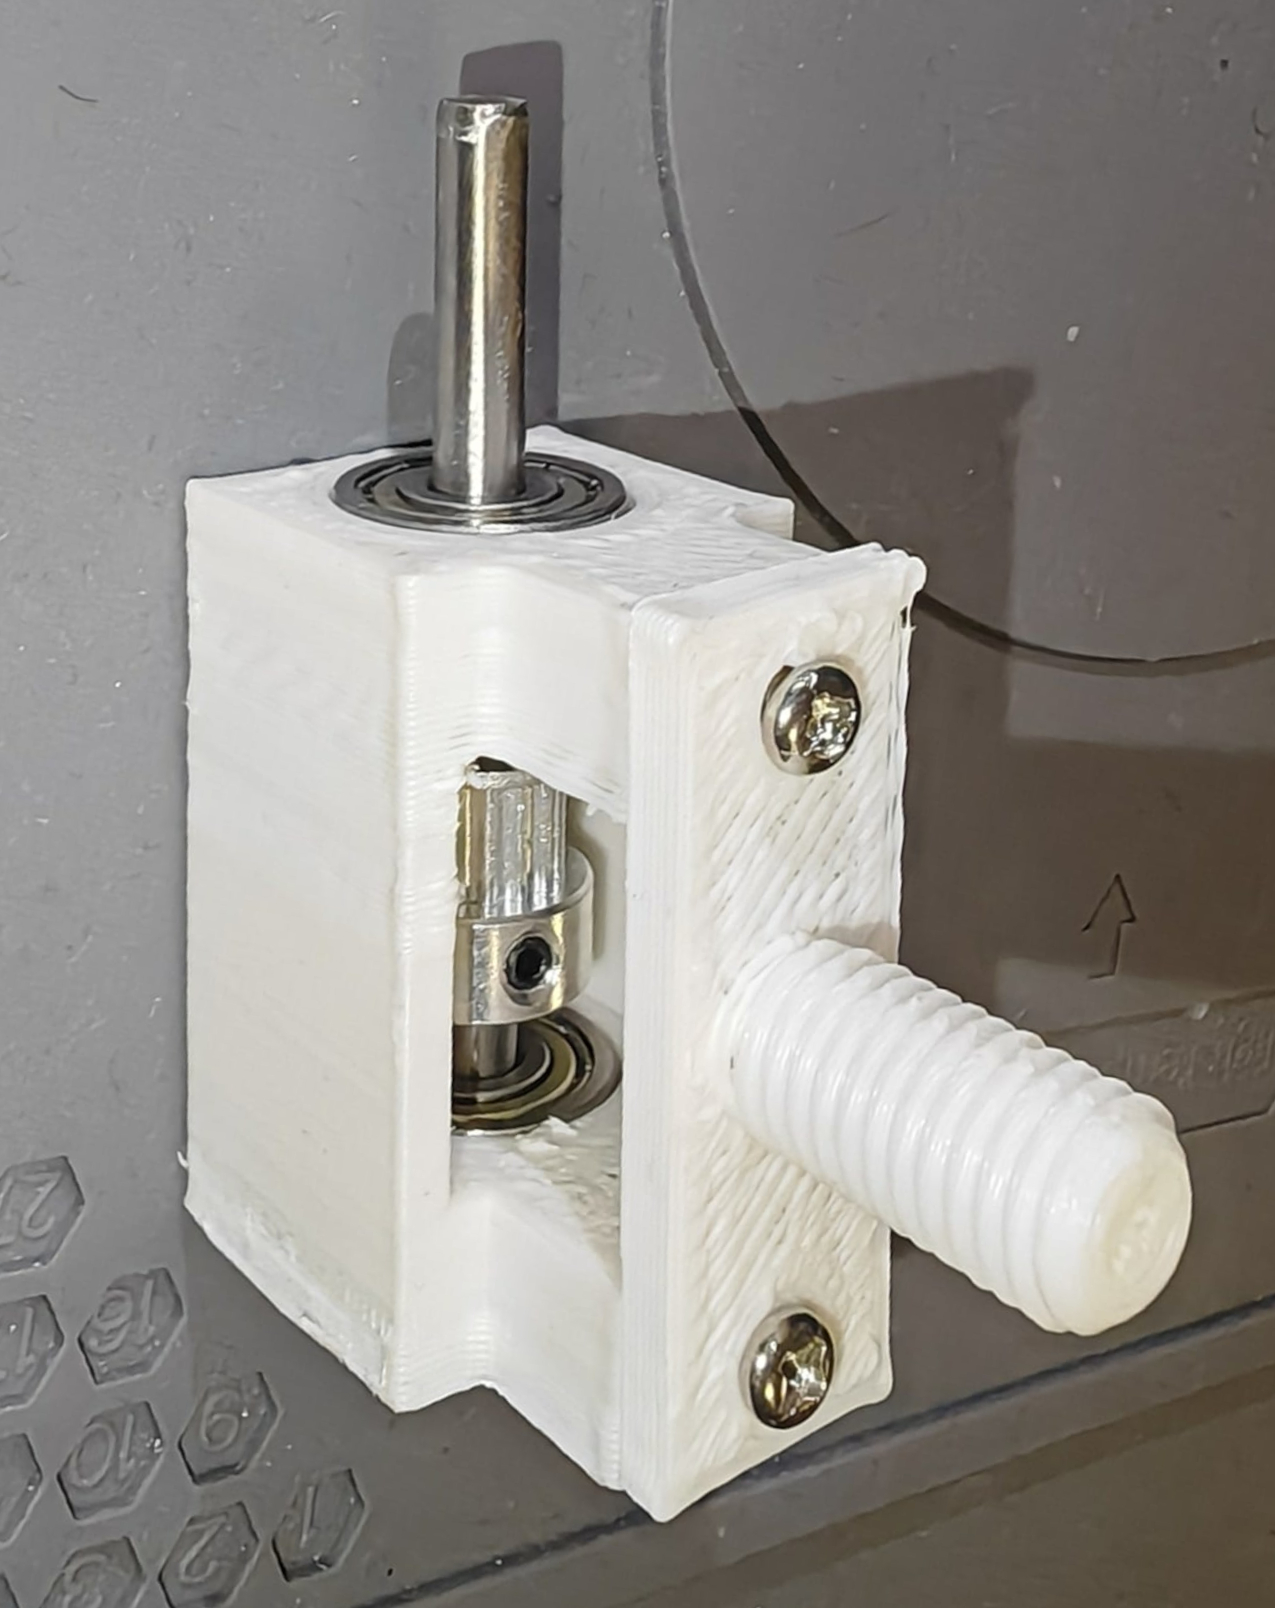
\includegraphics[height=7cm]{imgs/freecad/tensionermountreal.jpeg}
    \end{minipage}
    \hfill
    \caption{Motor and endstop mount, and belt tensioner}
    \label{fig:motorandtensioner}
\end{figure}

\textbf{Gantry}: The gantry rolls along the 2020 extrusion frame using v-rollers, and provides a mount for the sweeper arm and also triggers the endstop. The design is inspired by the Ender 3 as shown in \autoref{fig:ender3}, and is used to provide a smooth linear motion for the sweeper arm. Three M4 holes are present in the gantry to mount the v-rollers, and there are slots for the timing belt to be inserted into. Four M3 holes are present to mount the sweeper arm, and the gantry has a large bumper on the end to trigger the endstop. The gantry is shown in \autoref{fig:gantry}.

\begin{figure}[H]
    \begin{minipage}[h]{0.95\textwidth}
        \centering
        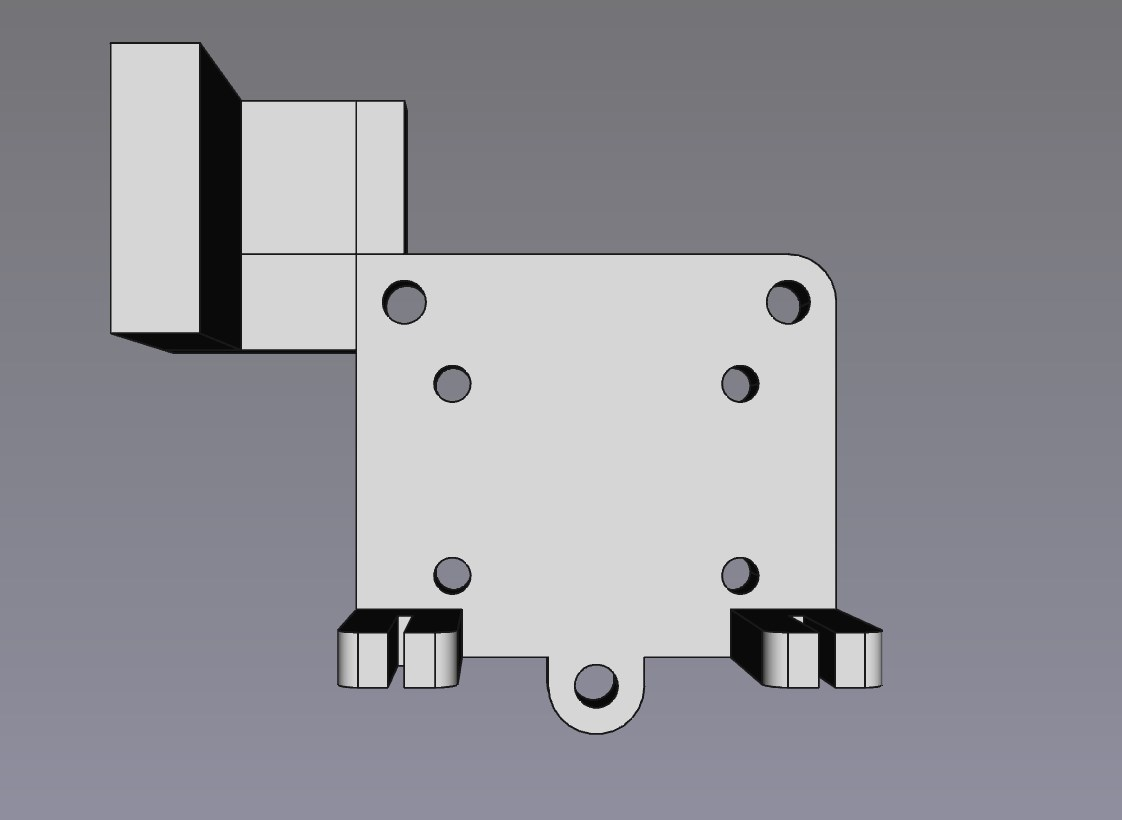
\includegraphics[height=8cm]{imgs/freecad/gantry.jpg}
        \caption{Gantry}
        \label{fig:gantry}
    \end{minipage}
\end{figure}

\textbf{Sweeper Arm}: The sweeper arm is the part of the system that pushes components off the conveyor belt into the sorting bins. In \autoref{fig:sweeperarm}, it attaches vertically to a mount using M3 screws and T-nuts, and mounts directly to the gantry. The v-rollers on the gantry are also visible for reference.

\begin{figure}[H]
    \begin{minipage}[h]{0.95\textwidth}
        \centering
        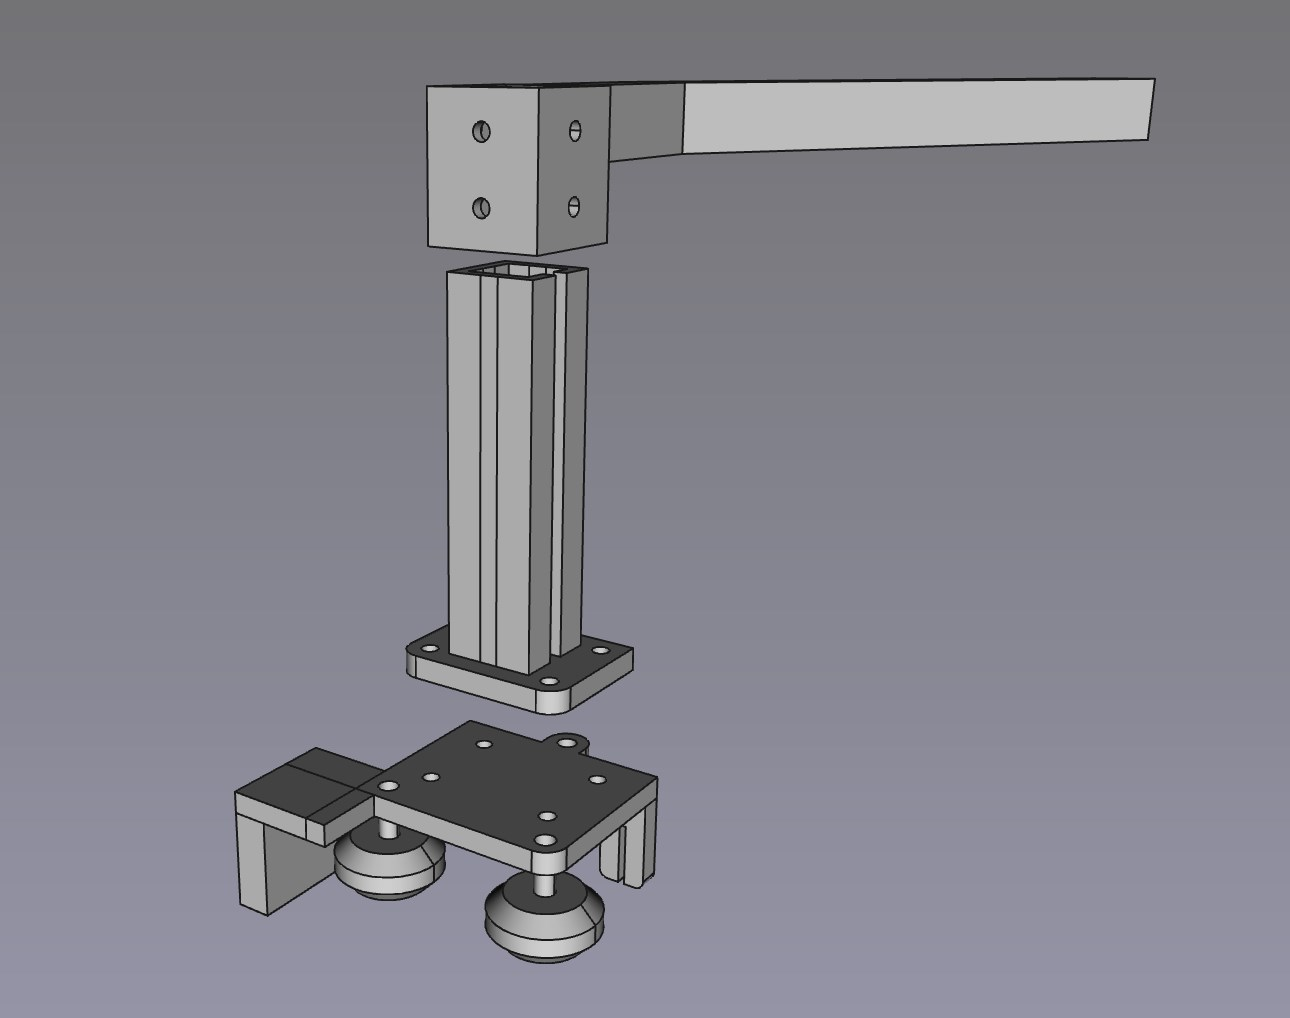
\includegraphics[height=8cm]{imgs/freecad/sweeperarm.jpg}
        \caption{Sweeper arm with v-rollers}
        \label{fig:sweeperarm}
    \end{minipage}
\end{figure}

\textbf{Bin}: The bin is used to catch components that are pushed off the conveyor belt by the sweeper arm. There are two parts to the bin; the bin itself and the extrusion mount. Originally, it was designed to have the extrusion mount be secured to the extrusion using M3 screws and T-nuts, but this was found to be unnecessary as the tight fit of the extrusion mount was sufficient to hold it in place. The bin is shown in \autoref{fig:bin}.

\begin{figure}[H]
    \begin{minipage}[h]{0.95\textwidth}
        \centering
        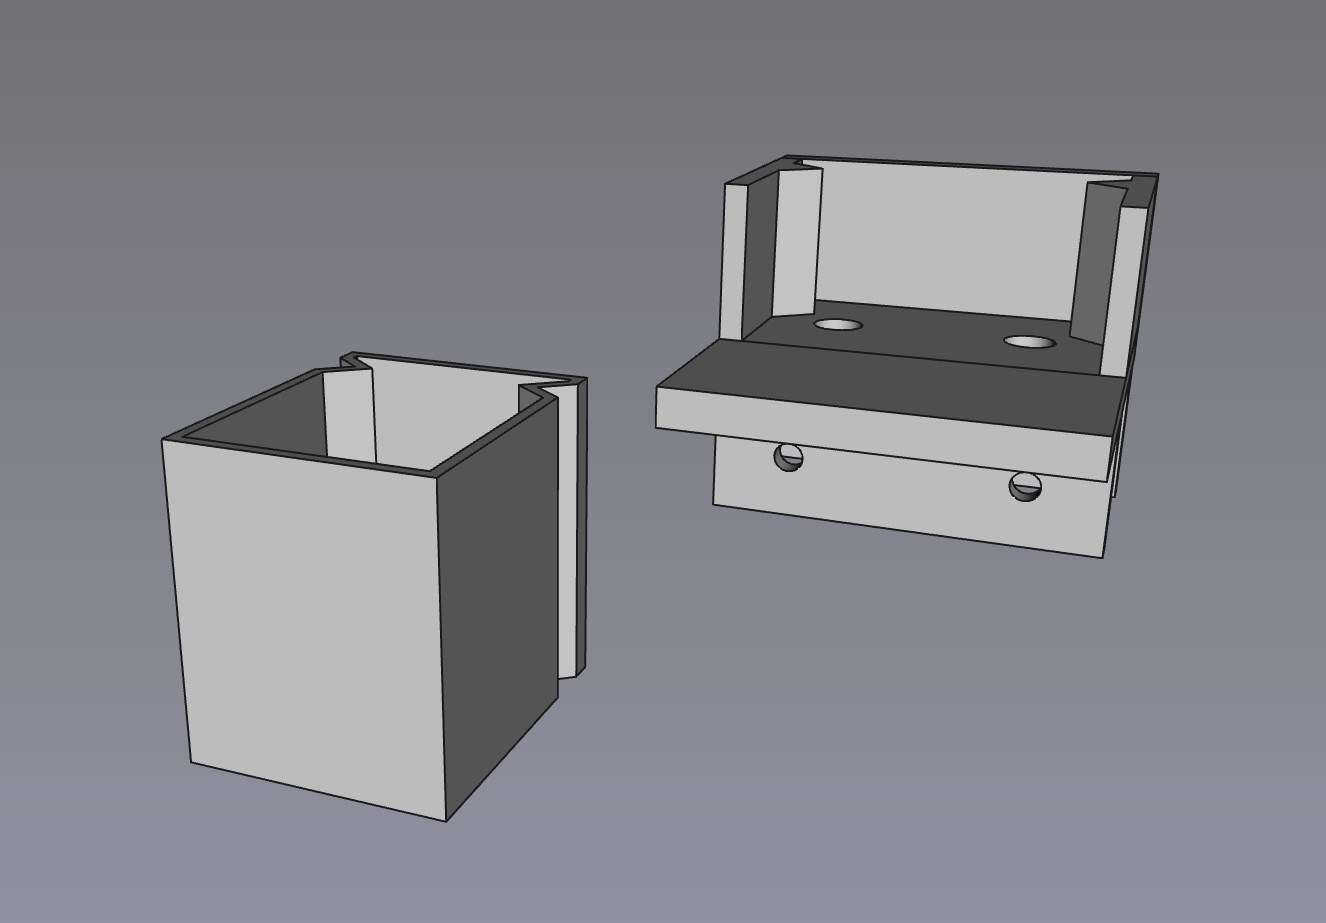
\includegraphics[height=8cm]{imgs/freecad/bin.jpg}
        \caption{Bin and extrusion mount}
        \label{fig:bin}
    \end{minipage}
\end{figure}

As shown in \autoref{fig:bin}, the bin simply slides into the extrusion mount due to the triangle insets, constraining it to only move directly up and down. There are also countersunk holes in the bin to allow for M3 screws to be inserted to secure the bin to the extrusion mount, but this was found to be unnecessary.
